\chapter{Discussion}

The \acrshort{ewc} paper is currently one of the most known approaches for overcoming catastrophic forgetting.
Their paper shows that it performs well on a permuted MNIST dataset with three sequential learning tasks.
\newline
Sadly the paper just delivers main facts and ideas behind the \acrshort{ewc} solution.
It has a lack of some important facts for understading their approaches and test benchmarks.
They do show the main idea, formula and advanatges by using them.
Nevertheless, they do not explain why they are using the \acrshort{fim}, in fact just the diagonal of the \acrshort{fim}.
Moreover, they do not documented helpful formulas, like the \acrshort{fim} or deeper calculation insights.
Even a code base is not available.
In the appendix are some parameters of their benchmarks documented.
Yet, their benchmarks for superviseed learning (Figure \ref{fig:ewc_permuted_example}) on the MNIST dataset are not reproducible.
They do not present a solution for a reasonable lambda value, learning rate or iterations for the second task.
Therefore, this article had to come up with its own benchmarks.
The benchmarks refer to the report \cite{cf_application_oriented_study} which includes an application-oriented study on the \acrshort{ewc} algorithm.
The network was given three hidden layers with 800 neurons.
This feature base is a proven structure for the MNIST problem.
The iterations and batch sizes are chosen from the study \cite{cf_application_oriented_study}.
This article increased the iterations for the permuted benchmark to analyze the surpassing of the $T_2$ accuracy to the complete dataset.
Lambda was initialized to $\lambda = \frac{1}{learning_rate \: T_2}$ by default.

Currently there are multiple implementations of \acrshort{ewc} available.
Most of them are created with PyTorch, a similar open-source machine learning library to Tensorflow.
Still, there are two solutions implemented in Tensorflow and available on Github
\footnote[1]{\url{https://github.com/ariseff/overcoming-catastrophic}}
\footnote[2]{\url{https://github.com/stokesj/EWC}}.
Both show a solution for a permuted MNIST on supervised learning but not a disjoint MNIST.
The more popular implementation\footnotemark[1] modifies the original algorithm.
For the \acrshort{fim} calulation it does not use the given labels from the dataset.
It generates new labels based on a randomization of the softmax probabilities.
% Moreover, the CrossEntropy loss funtion is not properly used for calculating the gradients.
% They avoid to negate the log from CE
The second implementation \footnotemark[2] is used in the report \cite{cf_application_oriented_study}.
As discovered in Section \ref{project_review_improvements} it built a workaround to be able to perform per-gradient calculations in Tensorflow.
This code base was the inspiration for the default lambda value.
\newline
The reimplementation of \acrshort{ewc} in Python and Tensorflow for this article omits these drawbacks and enables the algorithm for the modification \ref{project_review_improvements}.

The baseline showed that the \acrshort{ewc} algorithm works with the three benchmarks.
This \acrshort{ewc} algorithm (Figures \ref{fig:ewc_d9-1}, \ref{fig:ewc_d5-5}, \ref{fig:ewc_p10-10}) shows that it reduces catastrophic forgetting (Figures \ref{fig:catastrophic_forgetting_d91_example}, \ref{fig:catastrophic_forgetting_d55_example}).
However, it does not solve catastrophic forgetting for these benchmarks on the MNIST dataset.
\newline
The application-oriented study \cite{cf_application_oriented_study} discovered that \acrshort{ewc} is in some way effective against \acrlong{cf} for simple \acrshort{slt}s (D9-1 benchmark), but ineffective against \acrlong{cf} for more complex problems (D5-5 benchmark) \cite{cf_application_oriented_study}.
The complete dataset of their simple case (D9-1) has an accuracy after the second task of 71\% and a peak of 99\% \cite{cf_application_oriented_study}.
The results of this article (Figure \ref{fig:ewc_d9-1}) are with 85\% at the end and a peak of 93\% on the complete dataset similar to the paper.
In the case of D5-5 they can not register any sign of learning.
The second task has a end result of 31\% with a peak of 50\% \cite{cf_application_oriented_study}.
In comparison to these results, the benchmarks in this article (Figure \ref{fig:ewc_d5-5}) show that there is learning happending.
This benchmark substantiates an end result of 79\% with a peak of 82\%.
The third permuted benchmark in the reference paper \cite{cf_application_oriented_study} shows a peak of 100\% and an end result of 98\% at the second task training.
The result of this article is slightly lower with a peak and end result of 95\%.
\newline
It is interesting, that the benchmark types D9-1 and D5-5 with the implementation of this article just work with a lot lower learning rate of 0.00001 for $T_2$.
The learning rate of $T_1$ however is constantly 0.001.
\newline
The comparison of $T_2$ in Figure \ref{fig:ewc_d5-5} and $T_1$ in Figure \ref{fig:ewc_p10-10} shows that in the D5-5 benchmark it would be much easier to just train a new model with the complete MNIST dataset.
Because of the same iterations, batch size and a smaller learning rate of $T_1$ (in Figure \ref{fig:ewc_p10-10}) the perfromance of training the complete dataset instead of retraining with the \acrshort{ewc} algorithm would increase the accuracy.
As proposed in catastrophic forgetting (Section \ref{catastrophic_forgetting}) there will be a sacrifice of knowledge.
Though, these benchmarks are just a small representation of the problems in a largely scaled environment for models and datasets.
In this case MNIST just provides a simplification of the problem to be able to test an algorithm.
And it gives the ability to test several different parameters in a short amount of time and computation power.
So these benchmarks help to get a better understanding of the algorithm.
Of course, as described in the motivation (Section \ref{intro_motivation}) the goal is it to get to a artificial general intelligence, where an algorithm can behave like a human brain.
In order to get there the algorithm has to work on small datasets like MNIST as well.
But if the main challenges of \acrshort{ewc} are solved and the algorithm is ready for deployemnt, its first use would be in scenarios where multitask learning (Figure \ref{fig:intro_motivation_multitask_learning_paradigm}) is not an option.
Because as we can clearly see, \acrshort{ewc} reduces catastrophic forgetting, but does not solve it.

There are multiple ways to implement the \acrshort{ewc} algorithm with Python and Tensorflow.
The attached codebase \footnote{\url{https://github.com/florianwiech/incremental-machine-learning}} tried multiple implementations.
First implementations dealt with own datasets, iterators and network classes.
The advantage is that the developer has full control over the complete code.
Though, a big disadvantage is, that other developers need a lot of effort to understand the code.
This is why developers should use the given helper classes of included frameworks.
Most of the time they present a good documentation and other developers, who know the framework, are able to understand the code quite quickly.
Because of that reason the code was converted to built-in Tensorflow classes like the Dataset, Iterator and autoloading of the MNIST dataset.
This code sticks as close as possible to the Tensorflow provided classes and Low-Level API.
But along the way of converting the code to the Tensorflow classes, the developer of the code just lost a lot of control and the ability to see what exactly being calculated by just looking at the code.
This is a huge disadvantage with the built-in classes of Tensorflow.
\newline
Through the own implementation, the option between a \acrshort{fim} calculation and the \acrshort{gm} matrix is straightforward by adjusting the "batch\_matrix" variable.
Since both computations with a batch size of 1 are the same, the modification is applied when the batch size is higher than one.

The \acrshort{gm} was tested in the experiments.
The comparison between the baseline benchmarks and experiments with the modification look encouraging.
\newline
The \textbf{benchmark type D9-1} in the experiment Figure \ref{fig:exp_d9-1_bs1k} compared to the baseline Figure \ref{fig:ewc_d9-1} shows that the algorithm does work with the \acrshort{gm}.
The training samples $N$ of each batch are 1,000 samples.
The complete dataset in Figure \ref{fig:ewc_d9-1} has a peak of 93\% and an end accuracy of 86\% compared to Figure \ref{fig:exp_d9-1_bs1k} with a peak of 93\% and at the end 85\%.
\newline
To get deeper insights, Figure \ref{fig:dis_d91} shows the maximum calculated gradients of each layer in the matrices after the $T_1$ training.
The Parameters represent the set of weights and biases of theta for each layer.
It shows only the maximum values, because the minimum values are all approximatively zero and not meaningful.
It is interesting that in this case the maximum gradients of the \acrshort{gm} are often nearly 200\% the size of the \acrshort{fim} gradients.
But the learning of $T_2$ is in both cases similar.

\begin{figure}[H]
    \centering
    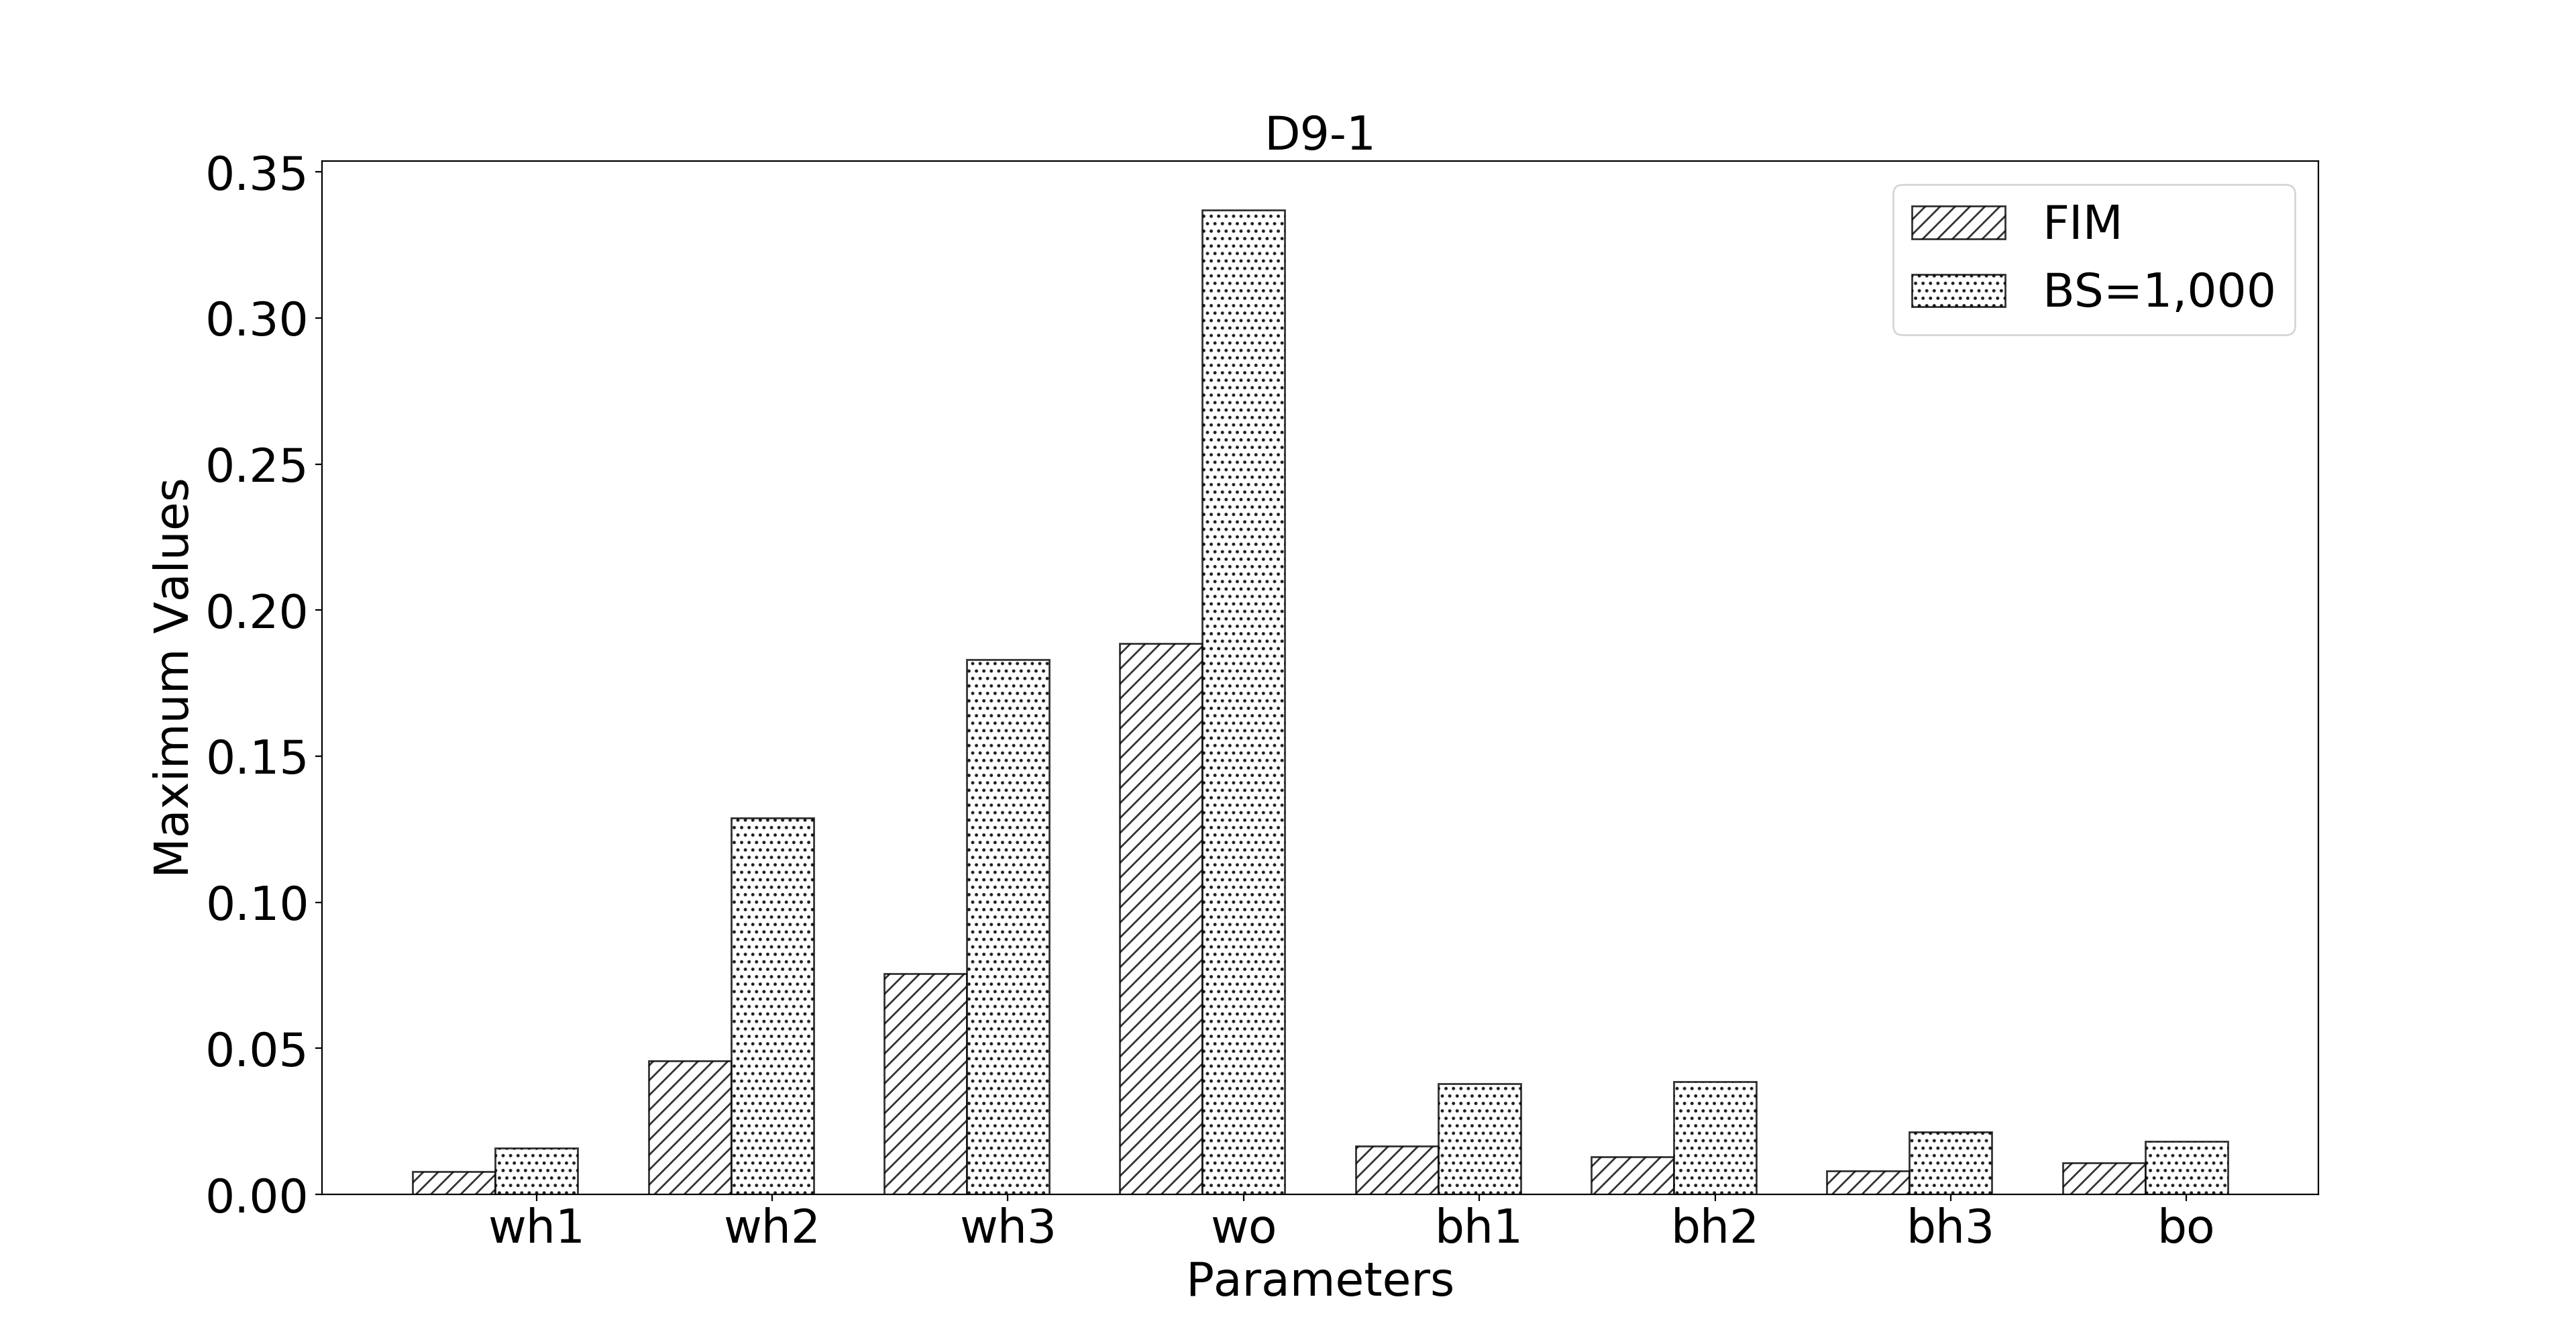
\includegraphics[width=\textwidth]{project/discussion/D91_grad_max}
    \caption{D9-1 Gradients}
    \label{fig:dis_d91}
\end{figure}

Figure \ref{fig:ewc_d5-5} compared to Figure \ref{fig:exp_d5-5_bs1k} in the \textbf{benchmark type D5-5} are very similar.
The result of the baseline was 79.52\% and of the experiment 79.45\%, with a peak of 81.52\% compared to the experiment of 81.16\%.
So both calculations do work with the difference that the \acrshort{gm} nearly took half the computation time of the original \acrshort{fim} calculation.
Figure \ref{fig:dis_d55} shows a composition of the extrem gradient values:

\begin{figure}[H]
    \centering
    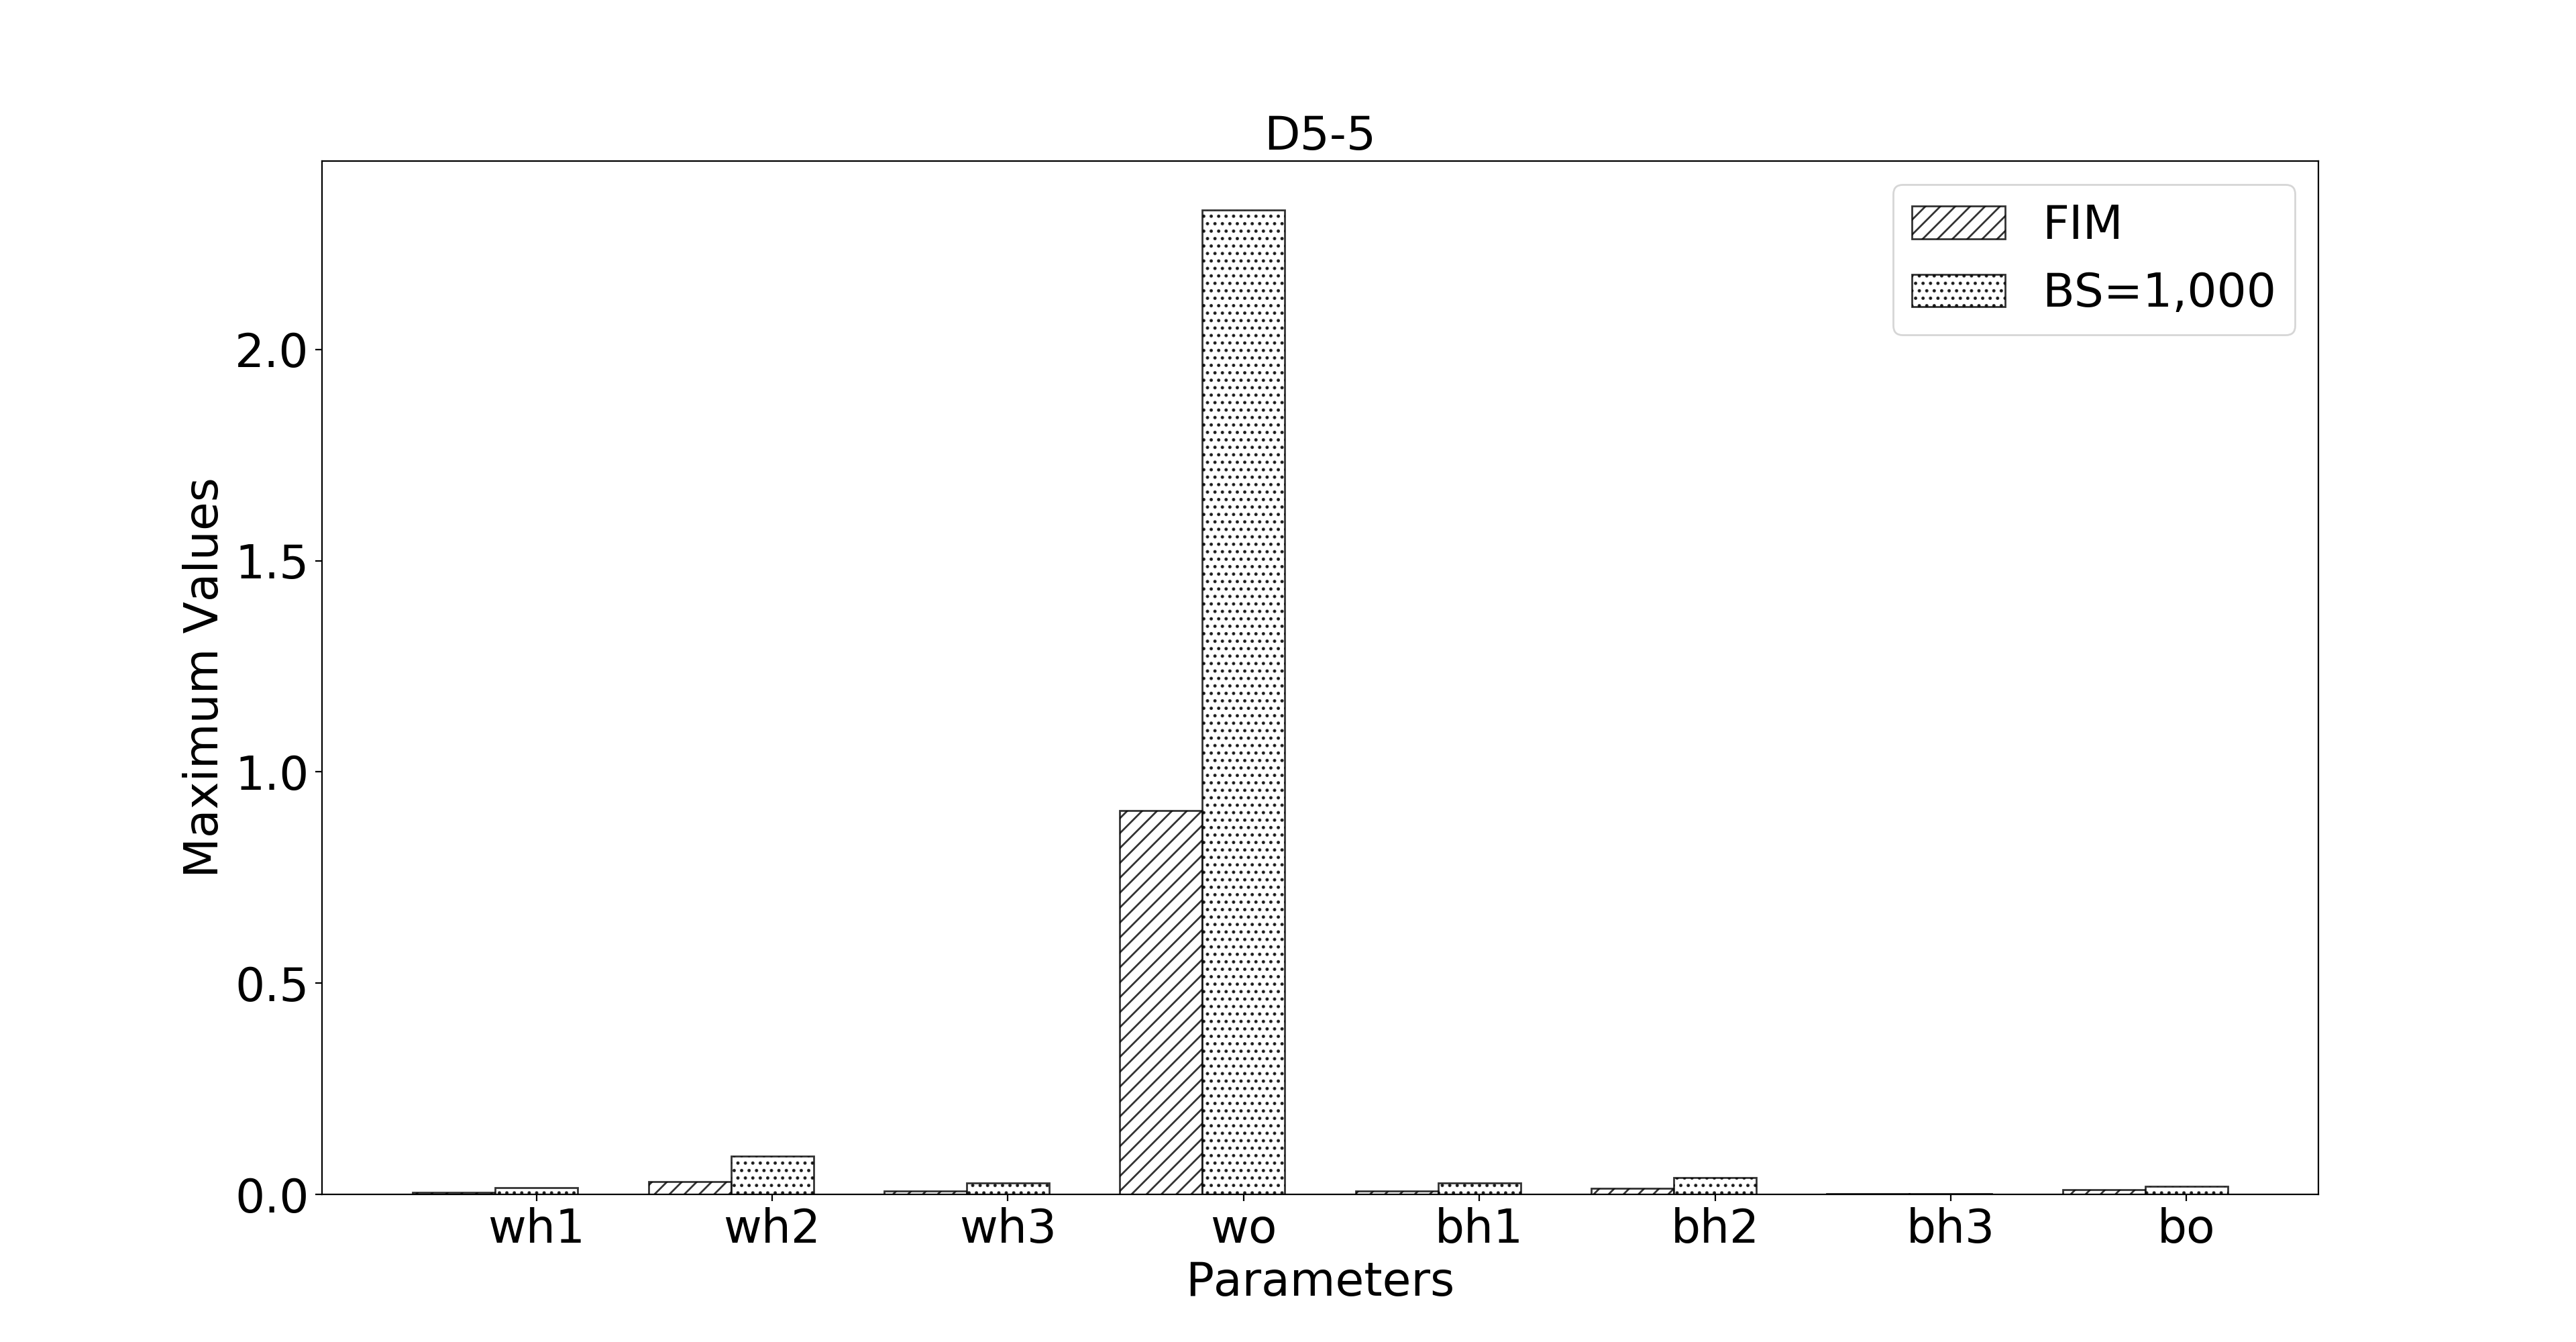
\includegraphics[width=\textwidth]{project/discussion/D55_grad_max}
    \caption{D5-5 Gradients}
    \label{fig:dis_d55}
\end{figure}

As well as the D9-1 benchmark, the gradient shows differences, yet, they do not make 
a difference at the $T_2$ training.
\newline
These gradient figures of the two benchmarks (Figure \ref{fig:dis_d91}, Figure \ref{fig:dis_d55}) do show differences in the comparison of every value.
Figure \ref{fig:dis_d91} exhibits more variations.
Both \acrshort{gm} matrices were calculated with an training set $N$ of 1,000 samples.
Nervertheless, their complete size of samples and the calculated weights and bias values differs.
The D9-1 benchmarks calculated 54 averaged gradients or 54,000 per-gradients and the D5-5 benachmark 30 averaged gradients or 30,500 per-gradients.

\textbf{Benchmark P10-10} with the baseline in Figure \ref{fig:ewc_p10-10} and the experiment Figure \ref{fig:exp_p10-10} shows that both $T_2$ trainings result in the same accuracy of the complete dataset with 90\%.
\newline
The several tests of the modification (Table \ref{table:exp_d10-10}) show, that multiple parameter combinations of learning rate and lambda have a auspicious result.
The best results for this task are with a higher learning rate and lambda value.
\newline
Figure \ref{fig:dis_d1010} shows the comparison of the gradient maximums.
As well as the other benchmarks, the maximum values of the \acrshort{gm} are much higher than the maximum values of the \acrshort{fim}.

\begin{figure}[H]
    \centering
    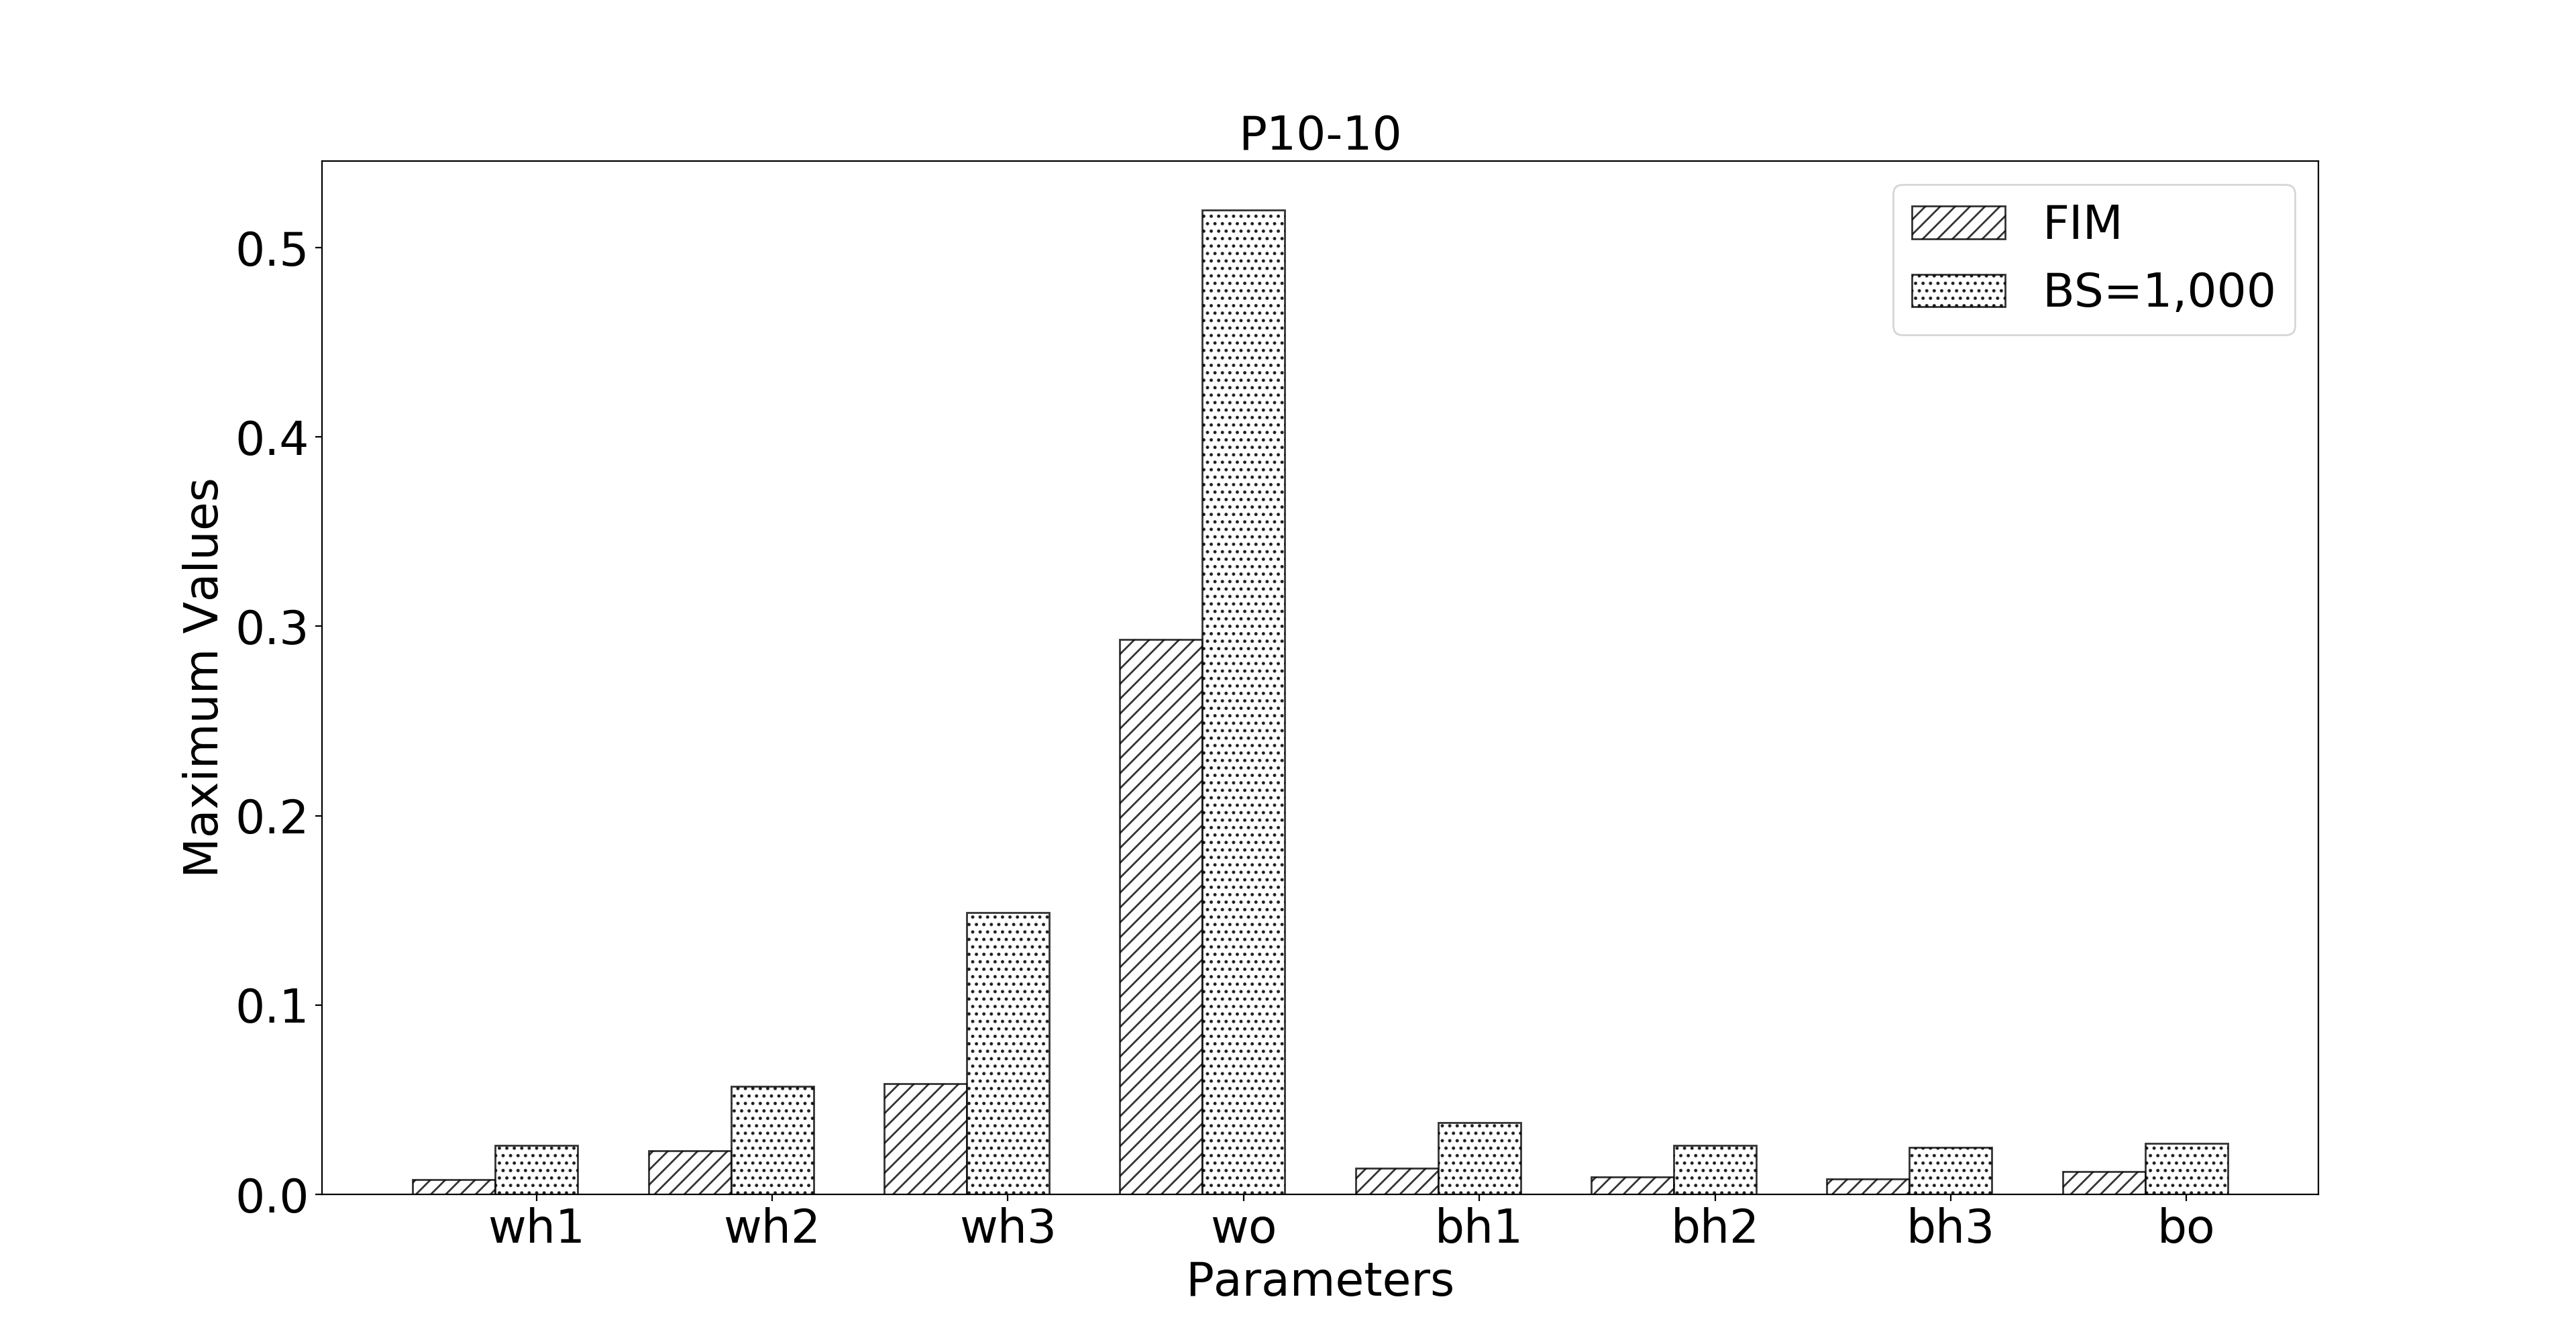
\includegraphics[width=\textwidth]{project/discussion/P1010_grad_max}
    \caption{P10-10 Gradients}
    \label{fig:dis_d1010}
\end{figure}

The promising benchmarks in this article worked with fixed iteration counts, learning rates and lambda value.
In the creation phase of the benchmarks, these three parameters had to be tested with multiple combinations.
Currently there is no solution, how to choose the quantity of iterations, learning rate or the lambda value.
So the developer needs to specify the importance of the \acrshort{ewc} appendix.
The reference implementation set it to $\lambda = \frac{1}{learning_rate \: T_2 }$, but we can clearly see in Table \ref{table:exp_d9-1} and Table \ref{table:exp_d5-5} of the D9-1 and D5-5 benchmarks, that this does not output the best result.
Even the comparison of these tables together show, that the chosen values for the best result differ from each other.
Regarding the tables it is important to note, that they just tested the learning rate and lambda value on a fixed iteration count.
But the number of iterations is a important component in the training process and can quickly collide with the other two parameters.
A solution for a iteration count might be the execution of a network test while training.
If the network finds a good solution while training it could presave it and train further.
If further trainings do not show a better result it can be terminated.
But this approach would definitly increase the training time, because of the increase of computations.
And it just could intercept useless training.
Overall a solution for the parameter choice problem might not be trivial.
\newline
For now the devleoper has to test multiple parameter combinations in order to find out, if this algorithm presents an useful outcome.
For every new task, a algorithm has to test multiple parameter choices in order get a feedback if there could be a promising result for the task.
This is a big problem and makes the algorithm really weak compared to the current multitask learning method.
The \acrshort{ewc} algorithm is not predictible to get any result, but multitask learning will present a result with a measurable period, which makes it the better choice for now.

\section{Conclusion}

The experiments and figueres from the discussion show that the introduced Gradient Matrix is a great simplification for the \acrshort{ewc} algorithm.
It delivers very similar results compared to the Fisher information matrix results from the baseline.
Since the Gradient matrix solves an issue with the \acrshort{ewc} algorithm and Tensorflow framework it is a better alternative for the Fisher information matrix.
The computation is decreased and the algorithm alleviates catastrophic forgetting, but does not prevent it.
However, the \acrshort{ewc} algorithm by itself deals with a lot of truble setting correct parameters.
Overall, the lack of knowledge about the correct value for these parameters makes the \acrshort{ewc} algorithm as described in their paper not useable for real-world scenarios.
So multitask learning will be the tool of choice for now.

\section{Outlook}

Further investigations should be made by searching a solution for the parameter problem.
This article presented a modification for the \acrshort{fim} which now should be tested with other popular datasets and continual learning algorithms that use this calculation as well.
% As discribed in the related work seciton (Section …), the IMM and NGD algorithms use the \acrshort{fim} as well.
Further tests could be, how much tasks the \acrshort{ewc} algorithm can store until catastrophic fogetting occurs drastically.

% Einsatz von EWC:
% wenn das parameter problem gelöst ist, sehe ich schon einsatzgebiete
% natürlich wird dieser algorithmus nicht 